\documentclass[twoside]{book}

% Packages required by doxygen
\usepackage{fixltx2e}
\usepackage{calc}
\usepackage{doxygen}
\usepackage{graphicx}
\usepackage[utf8]{inputenc}
\usepackage{makeidx}
\usepackage{multicol}
\usepackage{multirow}
\PassOptionsToPackage{warn}{textcomp}
\usepackage{textcomp}
\usepackage[nointegrals]{wasysym}
\usepackage[table]{xcolor}

% NLS support packages
\usepackage{hfont}

% Font selection
\usepackage[T1]{fontenc}
\usepackage{mathptmx}
\usepackage[scaled=.90]{helvet}
\usepackage{courier}
\usepackage{amssymb}
\usepackage{sectsty}
\renewcommand{\familydefault}{\sfdefault}
\allsectionsfont{%
  \fontseries{bc}\selectfont%
  \color{darkgray}%
}
\renewcommand{\DoxyLabelFont}{%
  \fontseries{bc}\selectfont%
  \color{darkgray}%
}
\newcommand{\+}{\discretionary{\mbox{\scriptsize$\hookleftarrow$}}{}{}}

% Page & text layout
\usepackage{geometry}
\geometry{%
  a4paper,%
  top=2.5cm,%
  bottom=2.5cm,%
  left=2.5cm,%
  right=2.5cm%
}
\tolerance=750
\hfuzz=15pt
\hbadness=750
\setlength{\emergencystretch}{15pt}
\setlength{\parindent}{0cm}
\setlength{\parskip}{0.2cm}
\makeatletter
\renewcommand{\paragraph}{%
  \@startsection{paragraph}{4}{0ex}{-1.0ex}{1.0ex}{%
    \normalfont\normalsize\bfseries\SS@parafont%
  }%
}
\renewcommand{\subparagraph}{%
  \@startsection{subparagraph}{5}{0ex}{-1.0ex}{1.0ex}{%
    \normalfont\normalsize\bfseries\SS@subparafont%
  }%
}
\makeatother

% Headers & footers
\usepackage{fancyhdr}
\pagestyle{fancyplain}
\fancyhead[LE]{\fancyplain{}{\bfseries\thepage}}
\fancyhead[CE]{\fancyplain{}{}}
\fancyhead[RE]{\fancyplain{}{\bfseries\leftmark}}
\fancyhead[LO]{\fancyplain{}{\bfseries\rightmark}}
\fancyhead[CO]{\fancyplain{}{}}
\fancyhead[RO]{\fancyplain{}{\bfseries\thepage}}
\fancyfoot[LE]{\fancyplain{}{}}
\fancyfoot[CE]{\fancyplain{}{}}
\fancyfoot[RE]{\fancyplain{}{\bfseries\scriptsize 생성시간 \+: 화 11월 25 2014 03\+:00\+:46, 프로젝트명 \+: L\+R\+U cache simulator, 생성자 \+:  Doxygen }}
\fancyfoot[LO]{\fancyplain{}{\bfseries\scriptsize 생성시간 \+: 화 11월 25 2014 03\+:00\+:46, 프로젝트명 \+: L\+R\+U cache simulator, 생성자 \+:  Doxygen }}
\fancyfoot[CO]{\fancyplain{}{}}
\fancyfoot[RO]{\fancyplain{}{}}
\renewcommand{\footrulewidth}{0.4pt}
\renewcommand{\chaptermark}[1]{%
  \markboth{#1}{}%
}
\renewcommand{\sectionmark}[1]{%
  \markright{\thesection\ #1}%
}

% Indices & bibliography
\usepackage{natbib}
\usepackage[titles]{tocloft}
\setcounter{tocdepth}{3}
\setcounter{secnumdepth}{5}
\makeindex

% Hyperlinks (required, but should be loaded last)
\usepackage{ifpdf}
\ifpdf
  \usepackage[pdftex,pagebackref=true]{hyperref}
\else
  \usepackage[ps2pdf,pagebackref=true]{hyperref}
\fi
\hypersetup{%
  colorlinks=true,%
  linkcolor=blue,%
  citecolor=blue,%
  unicode%
}

% Custom commands
\newcommand{\clearemptydoublepage}{%
  \newpage{\pagestyle{empty}\cleardoublepage}%
}


%===== C O N T E N T S =====

\begin{document}

% Titlepage & ToC
\hypersetup{pageanchor=false,
             bookmarks=true,
             bookmarksnumbered=true,
             pdfencoding=unicode
            }
\pagenumbering{roman}
\begin{titlepage}
\vspace*{7cm}
\begin{center}%
{\Large L\+R\+U cache simulator \\[1ex]\large 0.\+9.\+0 }\\
\vspace*{1cm}
{\large 다음에 의해 생성됨 \+:  Doxygen 1.8.8}\\
\vspace*{0.5cm}
{\small 화 11월 25 2014 03:00:46}\\
\end{center}
\end{titlepage}
\clearemptydoublepage
\tableofcontents
\clearemptydoublepage
\pagenumbering{arabic}
\hypersetup{pageanchor=true}

%--- Begin generated contents ---
\chapter{파일 색인}
\section{파일 목록}
다음은 모든 파일에 대한 목록입니다. (간략한 설명만을 보여줍니다) \+:\begin{DoxyCompactList}
\item\contentsline{section}{\hyperlink{main_8c}{main.\+c} }{\pageref{main_8c}}{}
\item\contentsline{section}{dkh/\hyperlink{code__analyze_8h}{code\+\_\+analyze.\+h} }{\pageref{code__analyze_8h}}{}
\item\contentsline{section}{dkh/\hyperlink{compiler_8h}{compiler.\+h} }{\pageref{compiler_8h}}{}
\item\contentsline{section}{dkh/\hyperlink{dk__kernel_8h}{dk\+\_\+kernel.\+h} }{\pageref{dk__kernel_8h}}{}
\item\contentsline{section}{dkh/\hyperlink{dk__list_8h}{dk\+\_\+list.\+h} }{\pageref{dk__list_8h}}{}
\item\contentsline{section}{dkh/\hyperlink{dk__str_8h}{dk\+\_\+str.\+h} }{\pageref{dk__str_8h}}{}
\item\contentsline{section}{dkh/\hyperlink{dk__tree_8h}{dk\+\_\+tree.\+h} }{\pageref{dk__tree_8h}}{}
\item\contentsline{section}{dkh/\hyperlink{errno_8h}{errno.\+h} }{\pageref{errno_8h}}{}
\item\contentsline{section}{dkh/\hyperlink{file__read_8h}{file\+\_\+read.\+h} }{\pageref{file__read_8h}}{}
\item\contentsline{section}{dkh/\hyperlink{hash_8h}{hash.\+h} }{\pageref{hash_8h}}{}
\item\contentsline{section}{dkh/\hyperlink{list_8h}{list.\+h} }{\pageref{list_8h}}{}
\item\contentsline{section}{dkh/\hyperlink{lru_8h}{lru.\+h} }{\pageref{lru_8h}}{}
\item\contentsline{section}{dkh/\hyperlink{print__msg_8h}{print\+\_\+msg.\+h} }{\pageref{print__msg_8h}}{}
\end{DoxyCompactList}

\chapter{파일 문서화}
\hypertarget{main_8c}{\section{main.\+c 파일 참조}
\label{main_8c}\index{main.\+c@{main.\+c}}
}
{\ttfamily \#include $<$stdlib.\+h$>$}\\*
{\ttfamily \#include $<$stdio.\+h$>$}\\*
{\ttfamily \#include $<$string.\+h$>$}\\*
{\ttfamily \#include $<$fcntl.\+h$>$}\\*
main.\+c에 대한 include 의존 그래프
\nopagebreak
\begin{figure}[H]
\begin{center}
\leavevmode
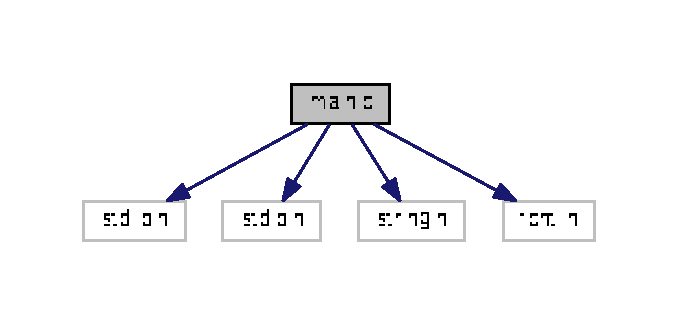
\includegraphics[width=326pt]{main_8c__incl}
\end{center}
\end{figure}
\subsection*{함수}
\begin{DoxyCompactItemize}
\item 
int \hyperlink{main_8c_a0ddf1224851353fc92bfbff6f499fa97}{main} (int argc, char $\ast$argv\mbox{[}$\,$\mbox{]})
\end{DoxyCompactItemize}


\subsection{함수 문서화}
\hypertarget{main_8c_a0ddf1224851353fc92bfbff6f499fa97}{\index{main.\+c@{main.\+c}!main@{main}}
\index{main@{main}!main.\+c@{main.\+c}}
\subsubsection[{main}]{\setlength{\rightskip}{0pt plus 5cm}int main (
\begin{DoxyParamCaption}
\item[{int}]{argc, }
\item[{char $\ast$}]{argv\mbox{[}$\,$\mbox{]}}
\end{DoxyParamCaption}
)}}\label{main_8c_a0ddf1224851353fc92bfbff6f499fa97}

%--- End generated contents ---

% Index
\newpage
\phantomsection
\addcontentsline{toc}{chapter}{색인}
\printindex

\end{document}
